% Options for packages loaded elsewhere
\PassOptionsToPackage{unicode}{hyperref}
\PassOptionsToPackage{hyphens}{url}
%
\documentclass[
]{book}
\usepackage{amsmath,amssymb}
\usepackage{lmodern}
\usepackage{ifxetex,ifluatex}
\ifnum 0\ifxetex 1\fi\ifluatex 1\fi=0 % if pdftex
  \usepackage[T1]{fontenc}
  \usepackage[utf8]{inputenc}
  \usepackage{textcomp} % provide euro and other symbols
\else % if luatex or xetex
  \usepackage{unicode-math}
  \defaultfontfeatures{Scale=MatchLowercase}
  \defaultfontfeatures[\rmfamily]{Ligatures=TeX,Scale=1}
\fi
% Use upquote if available, for straight quotes in verbatim environments
\IfFileExists{upquote.sty}{\usepackage{upquote}}{}
\IfFileExists{microtype.sty}{% use microtype if available
  \usepackage[]{microtype}
  \UseMicrotypeSet[protrusion]{basicmath} % disable protrusion for tt fonts
}{}
\makeatletter
\@ifundefined{KOMAClassName}{% if non-KOMA class
  \IfFileExists{parskip.sty}{%
    \usepackage{parskip}
  }{% else
    \setlength{\parindent}{0pt}
    \setlength{\parskip}{6pt plus 2pt minus 1pt}}
}{% if KOMA class
  \KOMAoptions{parskip=half}}
\makeatother
\usepackage{xcolor}
\IfFileExists{xurl.sty}{\usepackage{xurl}}{} % add URL line breaks if available
\IfFileExists{bookmark.sty}{\usepackage{bookmark}}{\usepackage{hyperref}}
\hypersetup{
  pdftitle={Modelación matemática},
  pdfauthor={Gerardo Martín},
  hidelinks,
  pdfcreator={LaTeX via pandoc}}
\urlstyle{same} % disable monospaced font for URLs
\usepackage{longtable,booktabs,array}
\usepackage{calc} % for calculating minipage widths
% Correct order of tables after \paragraph or \subparagraph
\usepackage{etoolbox}
\makeatletter
\patchcmd\longtable{\par}{\if@noskipsec\mbox{}\fi\par}{}{}
\makeatother
% Allow footnotes in longtable head/foot
\IfFileExists{footnotehyper.sty}{\usepackage{footnotehyper}}{\usepackage{footnote}}
\makesavenoteenv{longtable}
\usepackage{graphicx}
\makeatletter
\def\maxwidth{\ifdim\Gin@nat@width>\linewidth\linewidth\else\Gin@nat@width\fi}
\def\maxheight{\ifdim\Gin@nat@height>\textheight\textheight\else\Gin@nat@height\fi}
\makeatother
% Scale images if necessary, so that they will not overflow the page
% margins by default, and it is still possible to overwrite the defaults
% using explicit options in \includegraphics[width, height, ...]{}
\setkeys{Gin}{width=\maxwidth,height=\maxheight,keepaspectratio}
% Set default figure placement to htbp
\makeatletter
\def\fps@figure{htbp}
\makeatother
\setlength{\emergencystretch}{3em} % prevent overfull lines
\providecommand{\tightlist}{%
  \setlength{\itemsep}{0pt}\setlength{\parskip}{0pt}}
\setcounter{secnumdepth}{5}
\usepackage{booktabs}
\ifluatex
  \usepackage{selnolig}  % disable illegal ligatures
\fi
\usepackage[]{natbib}
\bibliographystyle{apalike}

\title{Modelación matemática}
\author{Gerardo Martín}
\date{2021-08-09}

\begin{document}
\maketitle

{
\setcounter{tocdepth}{1}
\tableofcontents
}
\hypertarget{preuxe1mbulo}{%
\chapter{Preámbulo}\label{preuxe1mbulo}}

\begin{center}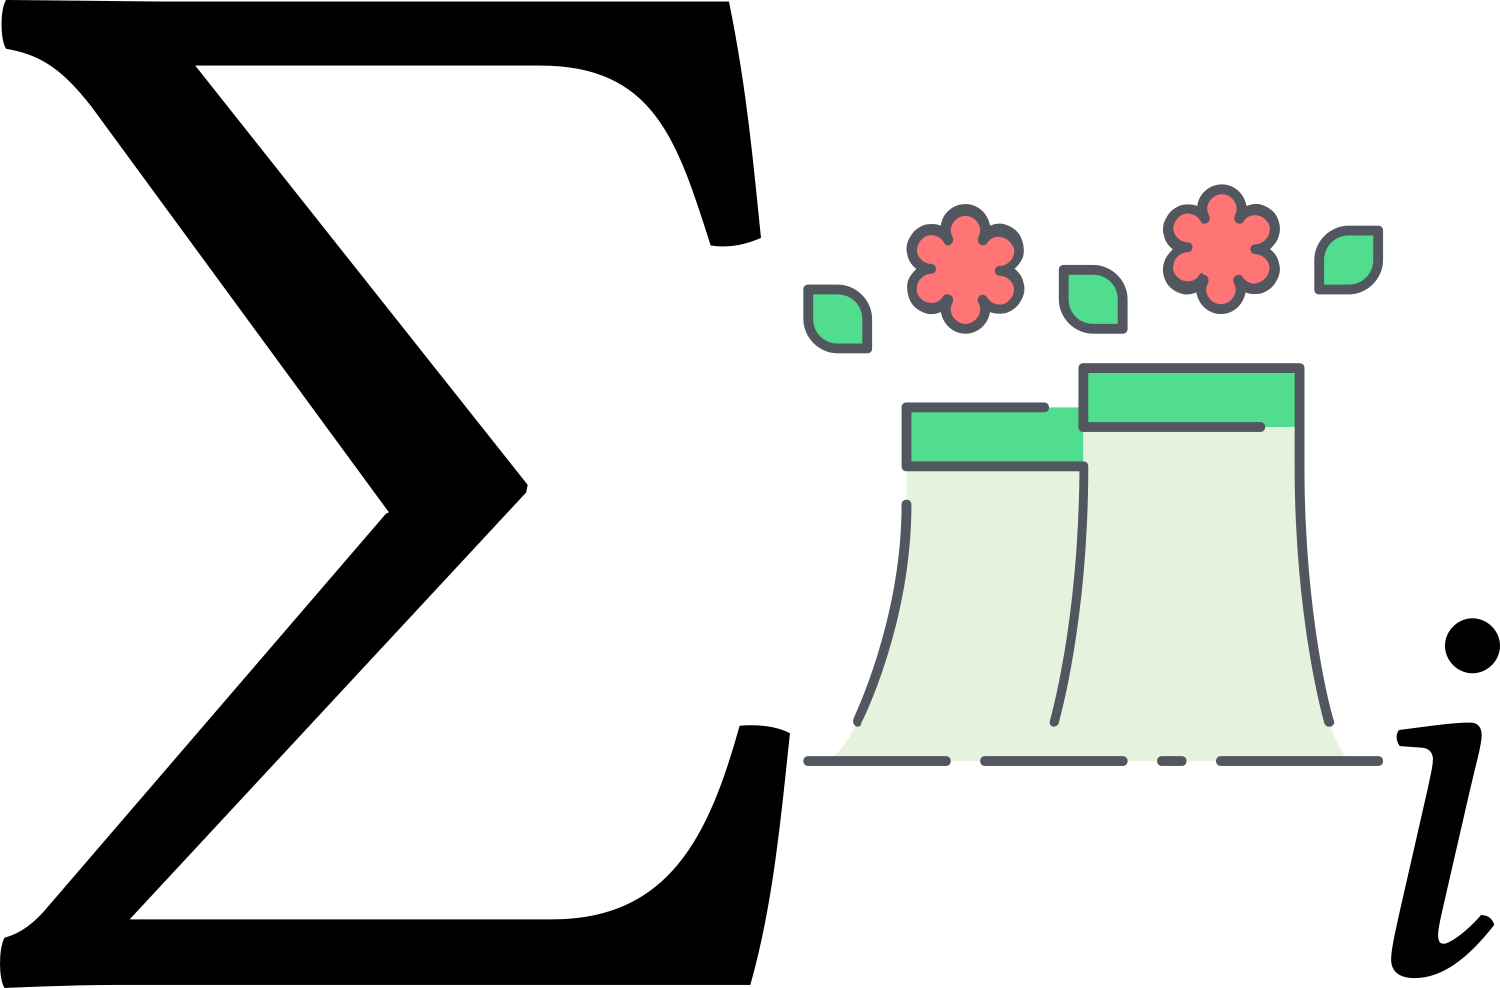
\includegraphics[width=20.83in]{logo} \end{center}

En el curso \textbf{Modelación matemática} aprenderemos a utilizar algunas herramientas matemáticas para analizar y entender los procesos de interés en ciencias ambientales. Los contenidos del índice se apegan al \href{Programa-curso.pdf}{programa completo del curso}, el cual se impartirá en los \href{Horario.pdf}{horarios normales establecidos}. Para conocer cuándo, cómo y qué temas se se impartirán puedes consultar la \href{Estrategia-docente.pdf}{estrategia docente}.

\hypertarget{criterios-de-evaluaciuxf3n}{%
\chapter{Criterios de evaluación}\label{criterios-de-evaluaciuxf3n}}

Las constribuciones a cada calificación parcial serán:

\begin{itemize}
\tightlist
\item
  Asistencia (25\%)
\item
  Trabajos de clase cumplidos (50\%)
\item
  Examen (25\%)
\item
  Participación (2 puntos extra máximo)
\end{itemize}

Cabe señalar, que la asistencia no corresponderá con su presencia en las sesiones sincrónicas, sino con el cumplimiento de los trabajos de clase. La participación se medirá tanto por participación directa en las sesiones sincrónicas como por el seguimiento que uds den a la clase por correo electrónico.

\hypertarget{cuxf3mo-se-daruxe1n-las-clases}{%
\section{¿Cómo se darán las clases?}\label{cuxf3mo-se-daruxe1n-las-clases}}

Trataré de apegarnos a los tiempos de actividades sincrónicas y asincrónicas establecidos en la \href{Estrategia-docente.pdf}{estrategia docente}, pero éstos son completamente flexibles. Una estrategia que me ha funcionado en cursos anteriores ha sido la de dedicar la última actividad sicrónica de la semana a resolver dudas, es en estas sesiones en las que hay muchas posibilidades de conseguir puntos de participación.

Todos los contenidos del curso, lecturas y presentaciones, se irán añadiendo a este sitio web conforme avanza el semestre. En el Google Classroom de la materia se irán anunciando las diferentes actividades y sesiones sincrónicas con anticipación suficiente. Igualmente, los examenes y resultados serán publicados a través de esta plataforma. A petición de uds, también se publicarán aquí los videos de las sesiones sincrónicas que tengamos, en especial para aquellos temas que sean mayor interés/dificultad/importancia. Los trabajos de práctica también se publicarán en Classroom.

\hypertarget{reglas-del-saluxf3n}{%
\section{Reglas del salón}\label{reglas-del-saluxf3n}}

Estas, obviamente, son particulares del modelo en línea, por lo tanto aquí van las reglas de zoom:

\begin{enumerate}
\def\labelenumi{\arabic{enumi}.}
\tightlist
\item
  Micrófonos apagados
\item
  Cámaras prendidas, exceptuando:
  2.1. Si su velocidad de internet lo dificulta
  2.2. Si tienen datos limitados
\item
  Hacer muchas preguntas
\item
  Decirme si paso algo por alto
\end{enumerate}

\hypertarget{contacto}{%
\section{Contacto}\label{contacto}}

Para reportar fallos, resolver dudas y peticiones especiales grupales o individuales por favor enviar correo electrónico a \href{mailto:gerardo.mmc@enesmerida.unam.mx}{\nolinkurl{gerardo.mmc@enesmerida.unam.mx}}.

\hypertarget{unidad-i-modelos-determinuxedsticos}{%
\chapter{Unidad I: Modelos determinísticos}\label{unidad-i-modelos-determinuxedsticos}}

\hypertarget{introducciuxf3n-a-la-modelaciuxf3n}{%
\section{Introducción a la modelación}\label{introducciuxf3n-a-la-modelaciuxf3n}}

Imaginemos a seis personas invidentes, con la tarea de encontrar qué es el objeto que está frente a ellas usando únicamente el tacto. En la parábola de los seis hombres ciegos, el objeto es un elefante, de modo que la imágen que cada uno de ellos se forma del objeto depende enteramente de la parte del elefante que están tocando.

\begin{figure}

{\centering 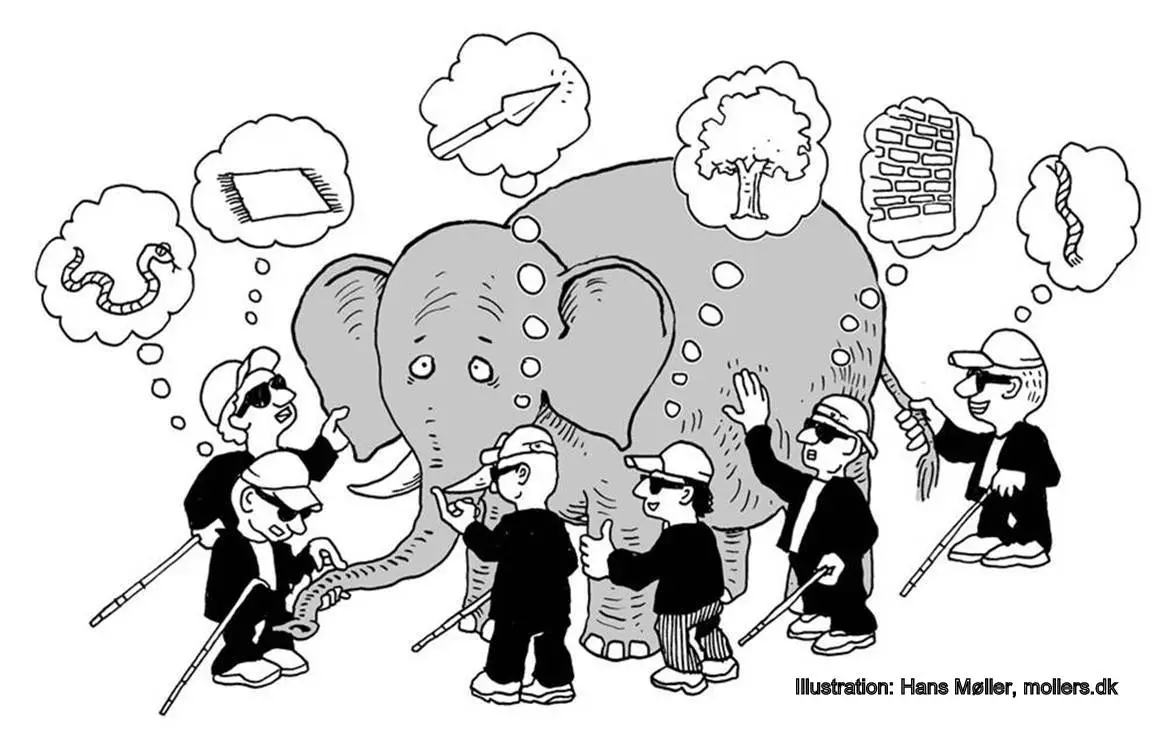
\includegraphics[width=16.17in]{Unidad-I/elefante} 

}

\caption{La parábola de los seis hombres ciegos inspeccionando un elefante.}\label{fig:unnamed-chunk-9}
\end{figure}

Quien toque los colmillos podrá pensar que se trata de una lanza, la trompa podría tratarse de una serpiente, la cola de una cuerda, las patas troncos de árbol y el cuerpo una pared. Es evidente que todas las hipótesis presentadas después de la inspección fueron erróneas, y que cuando estudiamos al mundo lo haremos igual, con la descripción de tan sólo una fracción de éste. Un séptimo hombre que pregunte a los otros seis qué fue lo que vieron podría formarse una imágen más completa del \emph{sistema} para proponer otra hipótesis: se trata de un objeto grande reposando sobre cuatro columnas con apéndices adelante y atrás.

Al estudiar los sistemas ecológicos, al igual que los ciegos, no sabremos que estamos frente a un elefante. Los sistemas ecológicos, al igual que los elefantes, también tienen componentes interconectados, y nosotros los ecólogos somos como los hombres ciegos, sólo podemos observar ciertas partes de los ecosistemas. En nuestro trabajo entonces, aprender a identificar y proponer hipótesis sobre cómo funcionan los sistemas ecológicos.

Las hipótesis propuestas por los seis hombres representan modelos, es decir simplificaciones del mundo que nos ayudan a entenderlo. Los modelos matemáticos son simplificaciones formales del mundo utilizando otro lenguaje, las matemáticas.

\hypertarget{funciones-buxe1sicas-y-su-representaciuxf3n-en-el-plano-cartesiano}{%
\section{Funciones básicas y su representación en el plano cartesiano}\label{funciones-buxe1sicas-y-su-representaciuxf3n-en-el-plano-cartesiano}}

\hypertarget{la-luxednea-recta}{%
\subsection{La línea recta}\label{la-luxednea-recta}}

Una línea recta se puede representar matemáticamente de varias maneras, la más común de ellas es por medio de una función. Una función, en cambio es una expresión matemática que indica una serie de operaciones (aritméticas por ejemplo), que serán aplicadas a un conjunto de números en sucesión (los números reales, p.~ej.) para producir otro conjunto. Así la, función lineal más sencilla puede ser:

\begin{equation}
    y(x) = x
\end{equation}

Lo que quiere decir que \(y\) es una función de \(x\), y cada valor de \(y\) será igual a cada valor de \(x\). En lenguaje matemático, el conjunto de números de \(x\) se llama el dominio, y \(y(x)\) el codominio. Algunas funciones lineales más complejas son:

\begin{equation}
    y(x) = ax
\end{equation}

donde \(a\) es una constante, lo que quiere decir que cada valor de \(y(x)\) será producido por el producto \(a \times x\). Finalmente, la expresión más común de una ecuación lineal es:

\begin{equation}
    y(x) = b + ax
\end{equation}

donde \(b\) también es una constante que se llama intercepto, y \(a\) es la pendiente, pues esta última determina la inclinación de la línea recta representada en el plano cartesiano.

\hypertarget{representaciones-gruxe1ficas-de-la-recta}{%
\subsubsection{Representaciones gráficas de la recta}\label{representaciones-gruxe1ficas-de-la-recta}}

Comencemos por dar un repaso del plano cartesiano. Este consiste de la representación de dos conjuntos de números reales en los que representamos una función, como una regla de correspondencia entre los valores de cada conjunto, de modo que a cada valor de \(x\) corresponde uno y sólo uno de los valores de \(y\). Cada conjunto se puede representar como una recta, y cuando éstas se disponen perperdiculares dan origen al plano.

\begin{figure}

{\centering 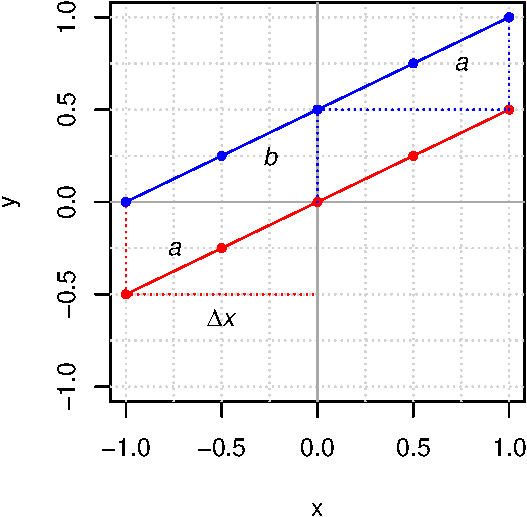
\includegraphics{Model-mate_files/figure-latex/unnamed-chunk-10-1} 

}

\caption{Ejemplo del plano cartesiado mostrando en rojo la correspondencia de valores para $y(x) = x$, donde los puntos corresponden a los pares de valores $(x = -1, y = -1), (-0.5, -0.5), (0, 0), (0.5, 0.5), (1, 1)$.}\label{fig:unnamed-chunk-10}
\end{figure}

Ahora veamos, con un ejemplo gráfico por qué la constante \(a\) recibe el nombre de \emph{pendiente}.

\begin{figure}

{\centering 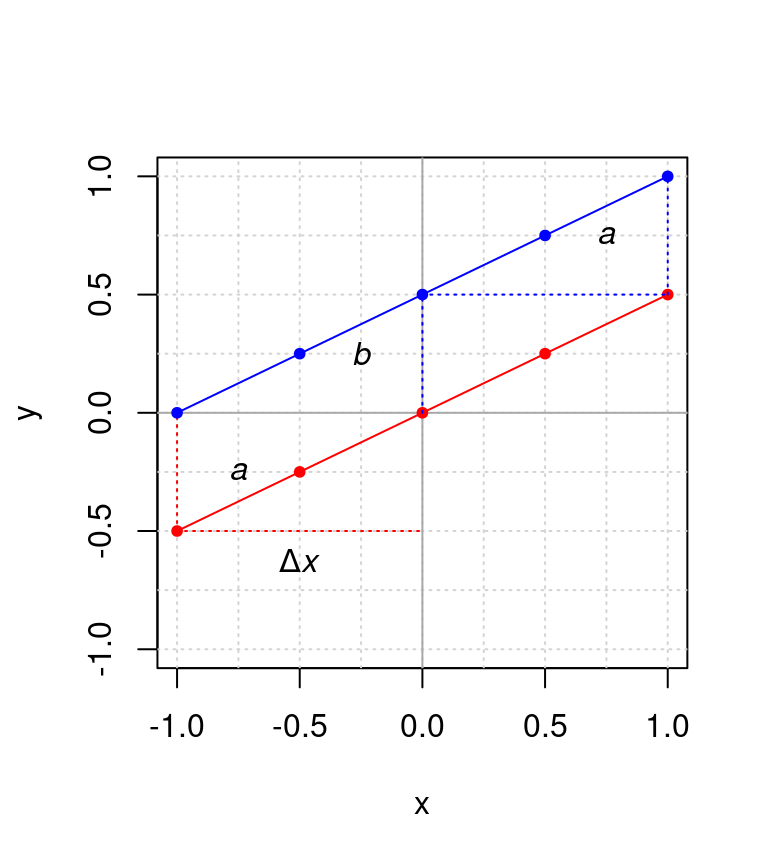
\includegraphics{Model-mate_files/figure-latex/unnamed-chunk-11-1} 

}

\caption{Gráficas de las funciones $y(x) = 0.5 x$ (en rojo) y $y(x) = 0.5 + 0.5 x$ (azul). Las líneas punteadas en colores indican el efecto de las constantes $a$ y $b$, mientas que Δ$x$ denota el cambio de una unidad de $x$.}\label{fig:unnamed-chunk-11}
\end{figure}

Como podemos ver, de manera más general, la línea recta es generada por una regla de correspondencia muy sencilla, un conjunto de valores \(X\) son multiplicados por un escalar \(a\), a los que se les puede añadir un \emph{intercepto} \(b\). El intercepto siempre es el valor de \(y(x)\) cuando \(x = 0\).

Ya se podrán imaginar que puede existir un sinnúmero de modelos lineales distintos, por ejemplo si \(y\) es una función de un gran número de conjuntos \(X\):

\begin{equation}
y(x_1, x_2, \dots, x_{n-1}, x_n) = b + a_1 x_1 + a_2 x_2 + \dots + a_{n-1} x_{n-1} + a_n x_n
\end{equation}

Gráficamente, estamos prácticamente limitados a explorar \(y(x_1, x_2)\), pero existen muchas herramientas matemáticas para entender modelos lineales más complejos que veremos más adelante. Estas herramientas y las implicaciones generales de la simplicidad del modelo lineal lo hacen uno de los modelos más útiles con que contamos para estudiar matemáticamente fenómenos dinámicos (que cambian de estado a lo largo del tiempo), como para estudiarlos de manera probabilística (con estadística). De hecho, el modelo lineal nos puede servir para entender modelos, como la parábola y el exponencial, que geométricamente no se parecen a la línea recta.

\hypertarget{la-paruxe1bola}{%
\subsection{La parábola}\label{la-paruxe1bola}}

Geométricamente, la parábola es muy distinta de la recta:

\begin{figure}

{\centering 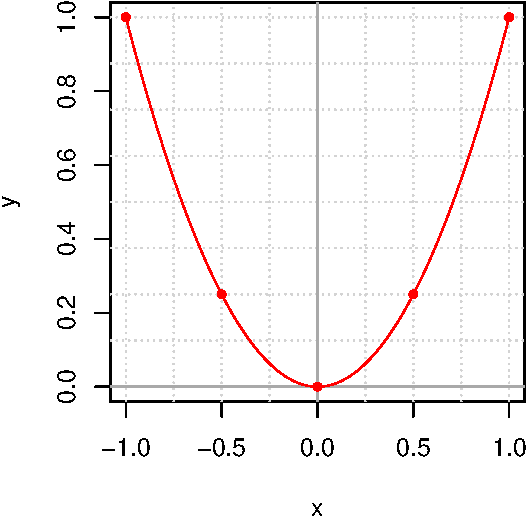
\includegraphics{Model-mate_files/figure-latex/parabola-1} 

}

\caption{Ejemplo del plano cartesiado mostrando en rojo la correspondencia de valores para $y(x) = x^2$, donde los puntos corresponden a los pares de valores $(x = -1, y = 1), (-0.5, 0.25), (0, 0), (0.5, 0.25), (1, 1)$.}\label{fig:parabola}
\end{figure}

La función matemática más sencilla que puede describir esta forma en el plano cartesiano es:

\begin{equation}
    y(x) = x^2
\end{equation}

Al igual que con los modelos lineales, las parábolas pueden representarse matemáticamente de otras formas más complejas:

\begin{itemize}
\tightlist
\item
  \(y(x) = a + bx + cx^2\)
\item
  \(y(x) = a + cx^2\)
\item
  \(y(x) = -x^2\)
\end{itemize}

Si uno es observador, se dará cuenta de que estas ecuaciones son muy similares a la recta, y es que es posible considerar que \(x^2\) se puede considerar como otro conjunto tal que \(x' = x^2\), resultando así en funciones perferctamente lineales:

\begin{itemize}
\tightlist
\item
  \(y(x) = a + bx + cx'\)
\item
  \(y(x) = a + cx'\)
\item
  \(y(x) = -x'\)
\end{itemize}

Entonce, lo que realmente distingue matemáticamente a una parábola de una recta, es la doble ocurrencia de cada valor de \(y\) para los distintos valores de \(x\):

\begin{figure}

{\centering 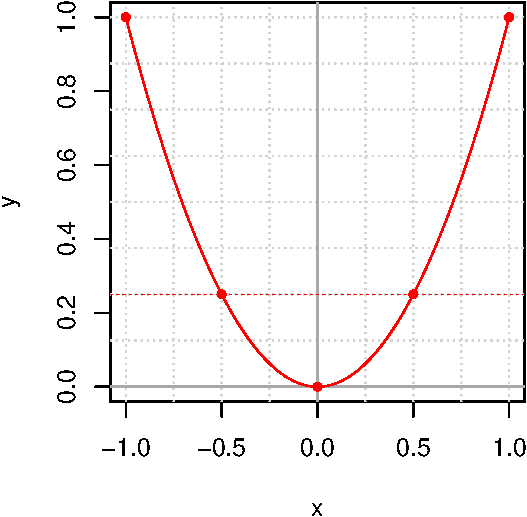
\includegraphics{Model-mate_files/figure-latex/parabola-2-1} 

}

\caption{Correspondencia de dos valores distintos de $x$ para el mismo valor de $y$}\label{fig:parabola-2}
\end{figure}

Cuando esto ocurre, las funciones tiene un solo punto a lo largo de todos los valores de \(x\), donde sólo va a ocurrir un valor único de \(y\). A estos puntos se les conocen como mínimos (par de valores con coordenadas \((0, 0)\) en la figura \ref{fig:parabola-2}). Los máximos, en cambio están ilustrados en la figura \ref{fig:parabola-3}, e igual corresponde al punto con coordenadas \((0, 0)\).

\begin{figure}

{\centering 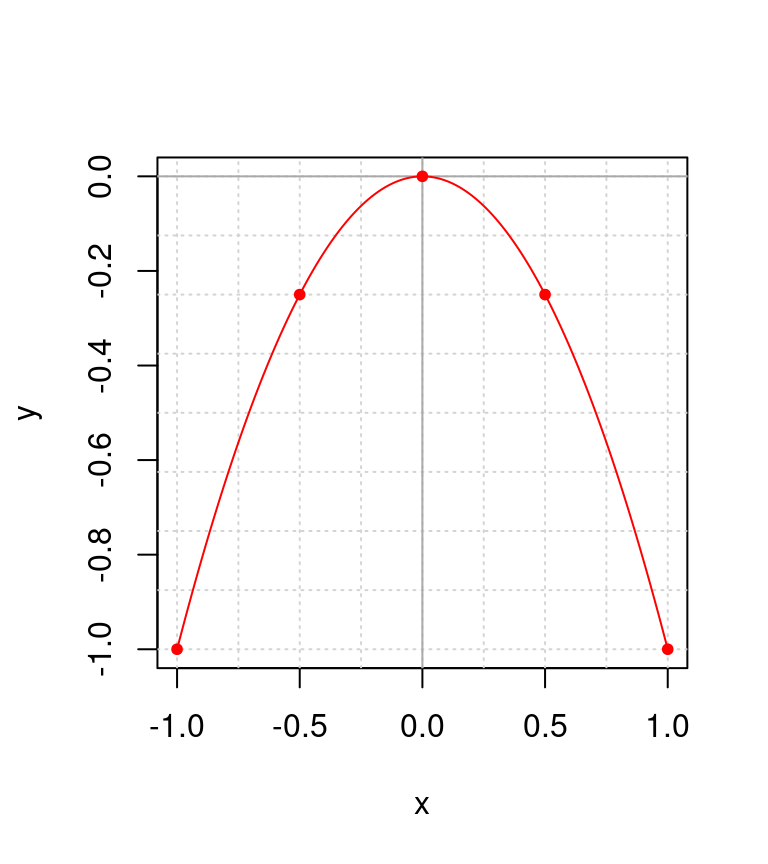
\includegraphics{Model-mate_files/figure-latex/parabola-3-1} 

}

\caption{Correspondencia de valores para $y = -x^2$.}\label{fig:parabola-3}
\end{figure}

En los modelos parabólicos más sencillos (\(y(x) = x^2, y(x) = -x^2\)), los puntos mínimos y máximos siempre estarán en las coordenadas \((x = 0, y = 0)\), pero es posible alterarlos. Por ejemplo en \(y(x) = 2 + x^2\), el mínimo estará en \((x = 0, y = 2)\). Para verificarlo resuelve \(y(x) = 2 + x^2\) para \(y(0)\), sustituyendo \(x\) por \(0\).

\hypertarget{ejercicio}{%
\subsubsection{Ejercicio}\label{ejercicio}}

A estas alturas, ya te podrás haber dado cuenta de ciertas propiedades de las parábolas, contesta las siguientes preguntas:

\begin{enumerate}
\def\labelenumi{\arabic{enumi}.}
\item
  ¿Qué tipo de punto único (mínimo o máximo) habrá en las siguientes parábolas?

  1.1. \(y(x) = 2 - x^2\)
  1.2. \(y(x) = 2x - 2x^2\)
  1.3. \(y(x) = 1 - x + 3x^2\)
  1.4. \(y(x) = x/2 - 4x^2/x\)
  1.5. \(y(x) = (5x)^2 - 3x + 1\)
\end{enumerate}

\hypertarget{cuxf3nicas}{%
\subsection{Cónicas}\label{cuxf3nicas}}

De manera muy general, una cónica es el conjunto de soluciones para una ecuación cuadrática cuando menos en dos variables. En este sentido, las parábolas, vistas en la sección anterior, son un tipo de cónica. Ejemplos:

\begin{enumerate}
\def\labelenumi{\arabic{enumi}.}
\tightlist
\item
  \(x^2 + y^2 = -1\)
\item
  \(x^2 + y^2 = 0\)
\item
  \(x^2 - y^2 = 0\)
\item
  \(xy - 1 = 0\)
\item
  \(x^2 - y = 0\)
\end{enumerate}

Debido a la generalidad de la definición de \emph{cónicas}, las ecuaciones 1-5 tienen una variedad de formas muy distintas, en comparación con las secciones de rectas y parábolas (Figura \ref{fig:conicas}). La mayoría de estas forman surgen como solución a la intersección de un plano bidimensional con una línea rotando sobre un eje definido dentro de ella en un espacio tridimencional (\href{https://www.mathplanet.com/Oldsite/media/28029/conic.png}{ver ejemplo})

\begin{figure}

{\centering 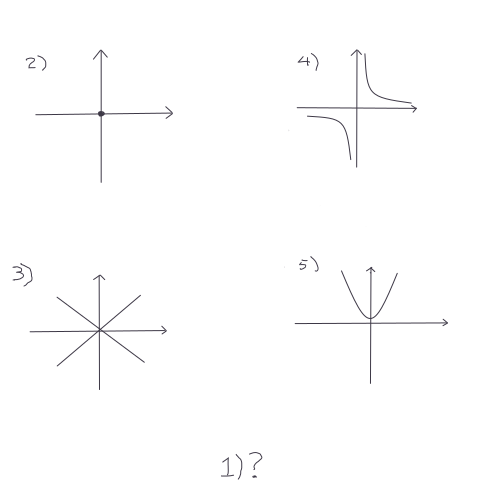
\includegraphics[width=6.93in]{Unidad-I/conicas} 

}

\caption{Representación gráfica de las ecuaciones 1-5.}\label{fig:conicas}
\end{figure}

\hypertarget{la-curva-normal}{%
\subsection{La curva normal}\label{la-curva-normal}}

En el curso de probabilidad y estadística, se acordarán, se mencionó repetidamente a la distribución normal. En cuestión de matemáticas, la distribución normal puede ser representada como una ecuación:

\begin{equation}
    y(x) = \frac{1}{\sigma \sqrt{2\pi}}e^{-\frac{(x-\mu)^2}{2\sigma^2}} \label{eq:normal}
\end{equation}

donde \(\mu\) es la media aritmética, \(\sigma^2\) es la varianza y \(x\) son todos los valores de la variable que observamos. Cuando tenemos datos de un experimento y los analizamos haciendo el cálculo del promedio estimamos justamente a \(\mu\) de la ecuación \eqref{eq:normal}, y al estimar la varianza obtenemos a \(\sigma^2\) de la misma ecuación. Como es importante notar, al hacer estos cálculos estamos asumiendo que nuestros datos tienen una distribución (un histograma) que puede ser descrita por la ecuación \eqref{eq:normal}.

Como vimos en la sección de parábolas, las funciones que no son monótonas (los valores de \(y\) no aumentan o disminuyen a lo largo de \(x\)), tienen un punto máximo o mínimo. La curva normal, tiene propiedades similares, aunque debido a la presencia de la función exponencial (\(e^{\dots}\)), los valores de \(y(x)\) \textbf{siempre serán positivos}. Por lo tanto, la curva normal tiene un punto máximo que corresponde a \(y(\mu)\), o sea, \(y\) alcanza su punto máximo cuando \(x=\mu\) (Figura \ref{fig:normal}).

\begin{figure}

{\centering 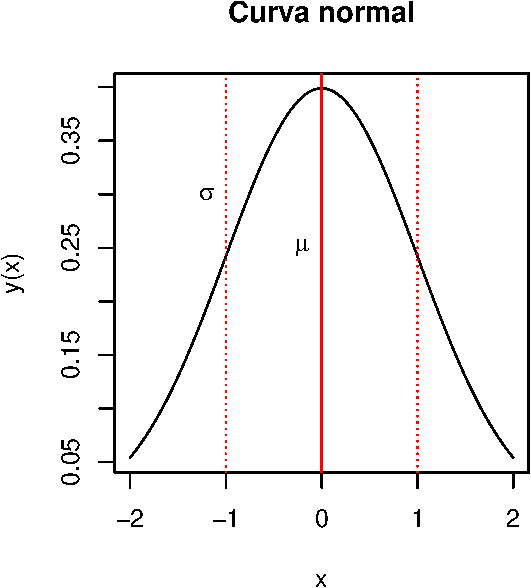
\includegraphics{Model-mate_files/figure-latex/normal-1} 

}

\caption{Representación gráfica de la curva normal.}\label{fig:normal}
\end{figure}

En estadística, esta función representa en el eje de las \(y\) la \emph{densidad} de la variable \(x\). Densidad se refiere a la proporción de observaciones de \(x\) dentro de un intervalo definido de \(x\). Por lo tanto, la curva normal, representa la probabilidad de observar ese valor de \(x\), de ahí que \(\mu\) sea el valor teórico más probable. En lo que respecta a \(\sigma^2\), éste representa qué tan concentrados estarán los valores de \(x\) alrededor de \(\mu\). Altos valores de \(\sigma\) se traducirán en baja concentración alrededor de \(\mu\) (Figura \ref{fig:vari}).

\begin{figure}

{\centering 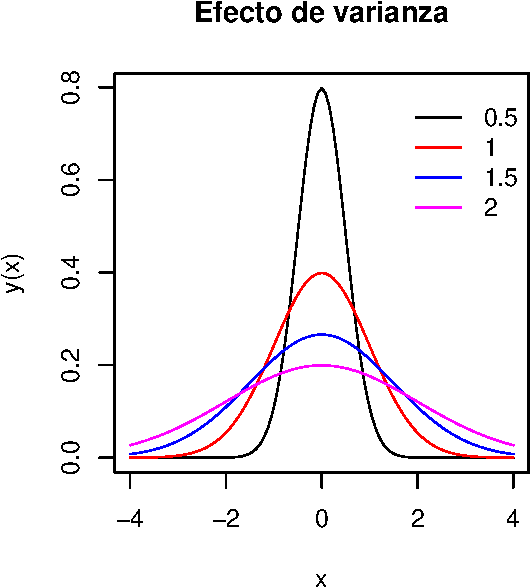
\includegraphics{Model-mate_files/figure-latex/vari-1} 

}

\caption{Efecto de  la varianza sobre la la dispersión alrededor de la media.}\label{fig:vari}
\end{figure}

\hypertarget{funciones-complementarias-y-su-representaciuxf3n-en-dos-y-tres-dimensiones}{%
\section{Funciones complementarias y su representación en dos y tres dimensiones}\label{funciones-complementarias-y-su-representaciuxf3n-en-dos-y-tres-dimensiones}}

\hypertarget{funciones-trigonomuxe9tricas}{%
\subsection{Funciones trigonométricas}\label{funciones-trigonomuxe9tricas}}

En esta sección revisaremos algunas de las funciones trigonométricas y cómo se representan en el plano cartesiano.

La trigonometría es una rama de las matemáticas que se comenzó a desarrollar a partir de la necesidad de medir distancias de manera indirecta. Por ejemplo, la distancia entre la luna y la tierra y la tierra y el sol, la distancia entre dos barcos, la distancia entre un barco y el puero más cercano. Las herramientas trigonométricas entonces se comenzaron a desarrollar utilizando la geometría de triángulos rectángulos. Aquí es preciso describir el teorema de los triángulos proporcionales, dados dos triángulos con ángulos internos idénticos y longitudes de lados diferentes, los cocientes de las longitudes de sus lados serán iguales (Figura \ref{fig:trian-prop}).

\begin{figure}

{\centering 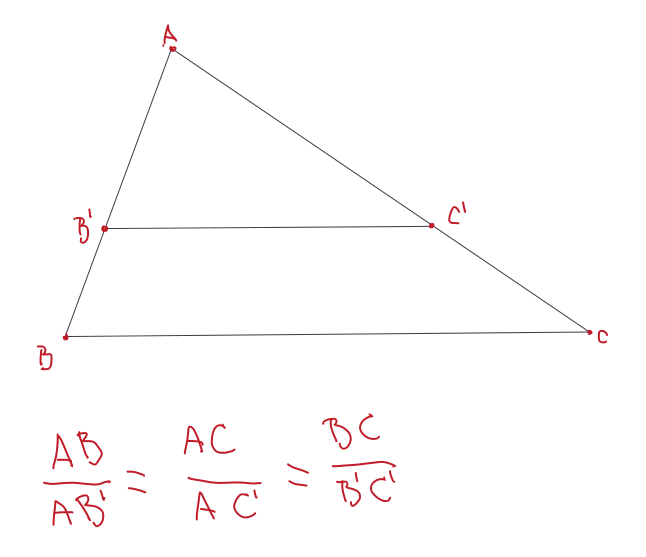
\includegraphics[width=8.97in]{Unidad-I/Trian-prop} 

}

\caption{El teorema de los ángulos proporcionales es la base para las fórmulas geométricas de las funciones trigonométricas.}\label{fig:trian-prop}
\end{figure}

De modo que sin importar las longitudes de los lados, los cocientes de las longitudes siempre serán iguales, lo cual se puede extender a todos los triángulos rectángulos, la base geométrica para la trigonometría. Aquí veremos entonces las funciones trognométricas básicas seno, coseno y tangente.

\hypertarget{nomenclatura-de-triuxe1ngulos-para-trigonometruxeda-buxe1sica}{%
\subsubsection{Nomenclatura de triángulos para trigonometría básica}\label{nomenclatura-de-triuxe1ngulos-para-trigonometruxeda-buxe1sica}}

Hay una serie de términos tradicionales que se emplean en trigonometría, los cuales utilizaremos a lo largo del curso. Se trata de los nombres que se dan a los lados y ángulos internos de un triángulo rectángulo. Por lo general, el triángulo rectángulo lo interpretaremos como una representación del plano cartesiano, de modo que los \textbf{catetos} corresponden a los ejes de las \(x\) y \(y\), y son los lados que forman un ángulo recto al cruzarse. El lado que los une en secante, es la \textbf{hipotenusa}. El ángulo que forma la hipotenusa con el eje de las \(x\) tradicionalmente recibe el nombre con la letra griega \(\theta\) (teta).

\begin{figure}

{\centering 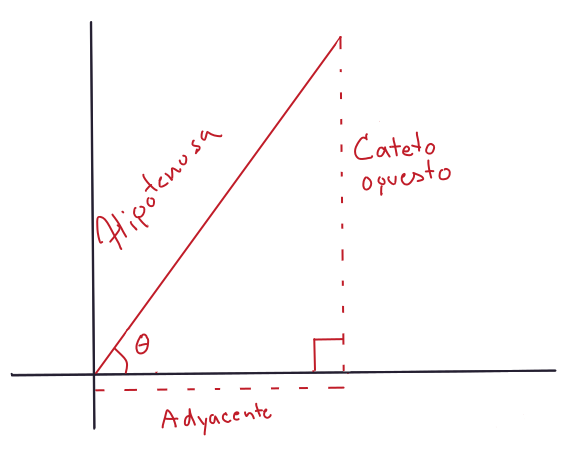
\includegraphics[width=7.86in]{Unidad-I/nomenclatura} 

}

\caption{Representación gráfica de las partes del triángulo y los nombres que reciben tradicionalmente en trigonometría plana.}\label{fig:nomen-trig}
\end{figure}

\hypertarget{las-funciones-trigonomuxe9tricas-buxe1sicas}{%
\subsubsection{Las funciones trigonométricas básicas}\label{las-funciones-trigonomuxe9tricas-buxe1sicas}}

Todas las funciones trigonométricas representan una descripción del ángulo \(\theta\) como el cociente de la longitud de dos lados del triángulo rectángulo de modo que:

\begin{enumerate}
\def\labelenumi{\arabic{enumi}.}
\tightlist
\item
  \(\sin(\theta) = \frac{\mathrm{Opuesto}}{\mathrm{Hipotenusa}}\)
\item
  \(\cos(\theta) = \frac{\mathrm{Adyacente}}{\mathrm{Hipotenusa}}\)
\item
  \(\tan(\theta) = \frac{\mathrm{Opuesto}}{\mathrm{Adyacente}}\)
\end{enumerate}

Para recordar las fórmulas de cada función podemos utilizar la mnemotecnia:

\begin{itemize}
\tightlist
\item
  \textbf{Seno}: SOH (Seno, Opuesto, Hipotenusa)
\item
  \textbf{Coseno}: CAH (Coseno, Adyacente, Hipotenusa)
\item
  \textbf{Tangente}: TOA (Tangente, Opuesto, Adyacente)
\end{itemize}

\hypertarget{la-luxednea-recta-como-modelo-universal}{%
\section{La línea recta como modelo ``universal''}\label{la-luxednea-recta-como-modelo-universal}}

\hypertarget{modelaciuxf3n-de-sistemas-sociales-y-ambientales}{%
\section{Modelación de sistemas sociales y ambientales}\label{modelaciuxf3n-de-sistemas-sociales-y-ambientales}}

\hypertarget{methods}{%
\chapter{Methods}\label{methods}}

We describe our methods in this chapter.

\hypertarget{applications}{%
\chapter{Applications}\label{applications}}

Some \emph{significant} applications are demonstrated in this chapter.

\hypertarget{example-one}{%
\section{Example one}\label{example-one}}

\hypertarget{example-two}{%
\section{Example two}\label{example-two}}

  \bibliography{book.bib,packages.bib}

\end{document}
